\documentclass[../main.tex]{subfiles}


\begin{document}
\raggedright

Web based systems are spread into various different languages with both positives and negatives. Java, .NET, PHP, ASP, Python, Ruby, ColdFusion are just a few of the most used language examples for web systems\cite{securelanguage}.


\begin{figure}[!htb]
        \center{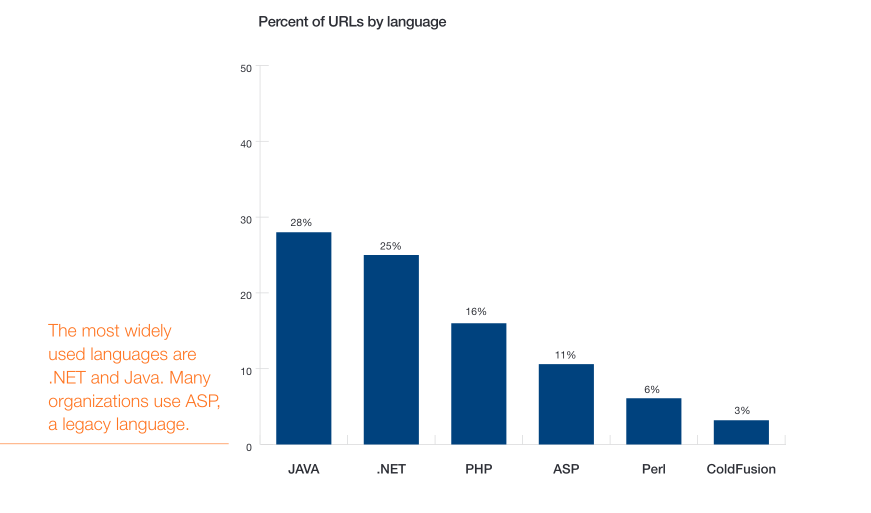
\includegraphics[scale=0.6]
        {images/mostLanguagesUsed.png}}
        \caption{\label{fig:my-label} Most widely used languages for Web Systems - WhiteHatSec\cite{WhiteHatSec}}
      \end{figure}


With all these languages, the highest priority would be to find a language which has Cyber Security as one of its strong points. .NET, Java, ASP, PHP all come with a high number of vulnerabilities as they are highly used\cite{securelanguage}. 

\begin{figure}[!htb]
        \center{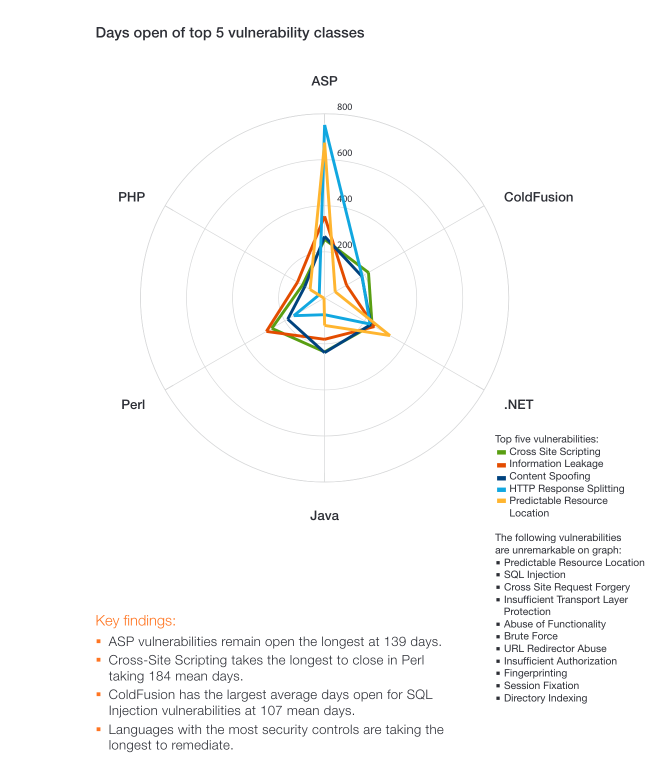
\includegraphics[scale=0.7]
        {images/languageAttacks.png}}
        \caption{\label{fig:my-label} Security Vulnerabilites in ASP, PHP, Perl, Java, .NET and ColdFusion - WhiteHatSec\cite{WhiteHatSec}}
      \end{figure}

This would then leave us with Python and Ruby which are both easy to code with and used widely. Using a web framework of the languages, Django(Python) or Ruby On Rails(Ruby) would be a smart idea because frameworks allow increased security as they are built for this and increase the efficiency and are cost effective\cite{djangovslaravel}. 


\end{document}
